\documentclass[12pt]{beamer}

\usepackage[T1]{fontenc}
\usepackage[utf8]{inputenc}
\usepackage{graphicx, tikz-qtree, caption, chronology}

\usetheme{CambridgeUS}
\usecolortheme{seagull}
\setbeamertemplate{title page}[default][shadow=false]
\setbeamertemplate{headline}{}
\setbeamertemplate{itemize items}[triangle]
\setbeamertemplate{footline}[frame number]{}
\setbeamertemplate{navigation symbols}{}

\title{Overview of hash-based\\digital signature schemes}
\author{Gustavo Zambonin\and Marcello Klingelfus}
\institute{
  
\includegraphics[scale=0.15]{ufsc}            \\ \vspace{-4mm}
  Federal University of Santa Catarina          \\
  Department of Informatics and Statistics      \\ \vspace{2mm}
  \texttt{\{gustavo.zambonin,marcello.klingelfus\}@grad.ufsc.br}
}
\date{}

\newcommand{\concat}{\, \vert \vert \,}
\newcommand{\hh}{$\mathcal{H}$}
\newcommand{\hash}[2][]{\mathcal{H}^{#1}(#2)}
\newcommand{\pad}{\vert \vert \, 0^*}

\begin{document}

\begin{frame}[plain,noframenumbering]
  \titlepage
\end{frame}

\begin{frame}
  \frametitle{Motivation}
  \begin{itemize}
    \setlength\itemsep{0.5em}
    \item Independent from number theory or algebraic problems
    \begin{itemize}
      \item Possibly `'post-quantum secure`'
    \end{itemize}
    \item For every digital signature scheme, one can use
        any hash function available
    \begin{itemize}
      \item Chosen according to specific needs (hardware, software)
    \end{itemize}
    \item One-way functions are necessary and sufficient for secure signatures
      \cite{Rompel:1990:OFN:100216.100269, cryptoeprint:2005:328}
  \end{itemize}
\end{frame}

\begin{frame}
  \frametitle{Foundations}
  \framesubtitle{Hash functions}
  \begin{equation*}
    \mathcal{H}: \{0, 1\}^{*} \longrightarrow \{0, 1\}^{n}
  \end{equation*}

  \begin{figure}
    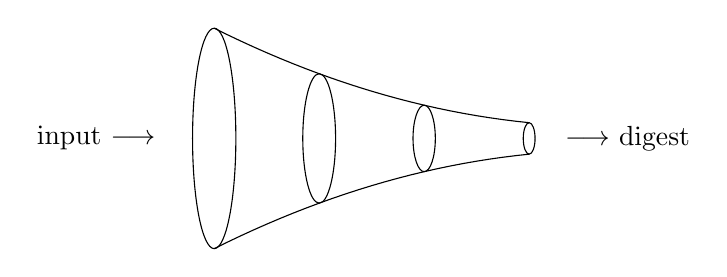
\begin{tikzpicture}
      \node at (-6.5, 0) {input $\longrightarrow$};
      \foreach \sgn in {+, -}
        \draw plot[domain=1:5] (-\x, {\sgn 1/20*(3+\x*\x)});
      \foreach \r in {1, 2.3333, ..., 5}
        \draw (-\r, 0) ellipse[x radius=(\r+.5)/20, y radius=1/20*(3+\r*\r)];
      \node at (0.25, 0) {$\longrightarrow$ digest};
    \end{tikzpicture}
  \end{figure}

  \begin{itemize}
    \item RIPEMD: $n \in \{128, 160, 256, 320\}$
    \item SHA-2, SHA-3, BLAKE: $n \in \{224, 256, 384, 512\}$
    \item Keccak: any $n$
  \end{itemize}
\end{frame}

\begin{frame}
  \frametitle{Foundations}
  \framesubtitle{}
  \begin{itemize}
    \item Provide authentication, integrity and non-repudiation
    \item Based on public-key cryptography
    \item Triple of probabilistic polynomial time algorithms
      \cite{Goldreich2004}
    \begin{itemize}
      \item Key generation ($\mathcal{G}$), signing ($\mathcal{S}$),
          verifying ($\mathcal{V}$)
    \end{itemize}
    \item There should exist a way to bind a signer to its key
  \end{itemize}

  \begin{figure}
    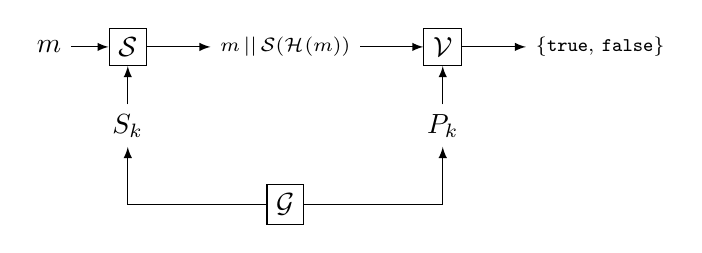
\begin{tikzpicture}
      \node (hm) at (-1, 0) {$m$};
      \node (sk) at (0, -1) {$S_{k}$};
      \node (pk) at (4, -1) {$P_{k}$};
      \node (ds) at (2, 0) {\scriptsize{$m \concat \mathcal{S}(\hash{m})$}};
      \node (res) at (6, 0) {\scriptsize\{\texttt{true}, \texttt{false}\}};
      \node[draw] (sig) at (0, 0) {$\mathcal{S}$};
      \node[draw] (ger) at (2, -2) {$\mathcal{G}$};
      \node[draw] (ver) at (4, 0) {$\mathcal{V}$};
      \draw[-latex] (ger) to (0, -2) to (sk);
      \draw[-latex] (ger) to (4, -2) to (pk);
      \draw[-latex] (sk) -- (sig);
      \draw[-latex] (hm) -- (sig);
      \draw[-latex] (sig) -- (ds);
      \draw[-latex] (ds) -- (ver);
      \draw[-latex] (pk) -- (ver);
      \draw[-latex] (ver) -- (res);
    \end{tikzpicture}
  \end{figure}
\end{frame}

\begin{frame}
    \frametitle{AES}
    \begin{itemize}
        \item Uma cifra de blocos simétrica e reversivel
        \item Suas operações são definidas sobre um corpo finito
        $\mathbb{F}_{2^{8}}$
        \item Sua chave tem tamanho $n = \{128,192,256 \}$
    \end{itemize}
    
\end{frame}

\begin{frame}
    \frametitle{AES}
    \framesubtitle{Funcionamento}
    \begin{itemize}
        \item Cada bloco é representado por uma matriz de estado $A$ de dimensões $4 \times 4$
        \item Seu funcionamento é constituido de multiplas iterações das seguintes operações em $A$, em relação a chave referente iteração a atual:
        \begin{itemize}
            \item\textsc{SubBytes}
            \item\textsc{ShiftRows}
            \item\textsc{MixColumns}
            \item\textsc{AddRoundKey}
        \end{itemize}
        \item A chave utilizada em cada iteração é obtida através de uma rotina de expansão da chave, denominada \textsc{KeyExpansion}
    \end{itemize}
\end{frame}

\begin{frame}
    \frametitle{AES}
    \framesubtitle{Operações}
    
\end{frame}

\begin{frame}
  \frametitle{One-time signature schemes}
  \begin{itemize}
    \item Key pair shall be used only once
    \item Lamport-Diffie (LD-OTS)
    \begin{itemize}
      \item First hash-based scheme
      \item Arbitrary-length messages can be signed, one bit at a time
    \end{itemize}
    \item Winternitz (WOTS)
    \begin{itemize}
      \item Multiple bits are signed simultaneously
      \item Generalization of LD-OTS
      \item Tradeoff between performance and signature size
    \end{itemize}
    \item HORS
    \begin{itemize}
      \item Few-time scheme, security decreases with each signature
      \item HORST --- HORS with trees
    \end{itemize}
  \end{itemize}
\end{frame}

\begin{frame}
  \frametitle{Winternitz OTS}
  \framesubtitle{Key generation step}
  Let $w \in \mathbb{N}, w > 1$ be the Winternitz tradeoff
  parameter. Then,
   \begin{align*}
       t_1 &= \left\lceil \frac{n}{w} \right\rceil \\
       t_2 &= \left\lceil
       \frac{\lfloor log_2 t_1 \rfloor + 1 + w}{w} \right\rceil \\
         t &= t_1 + t_2
   \end{align*}
   The private and public keys are, respectively,
   \begin{align*}
     S_k &= (y_{t - 1}, \dots, y_{0})
       \stackrel{\$}{\longleftarrow} \{0,1\}^n \\
     P_k &= (\hash[2^w - 1]{y_{t - 1}}, \dots, \hash[2^w - 1]{y_0})
   \end{align*}
\end{frame}

\begin{frame}
  \frametitle{Winternitz OTS}
  \framesubtitle{Signing step}
  The hash chain exponents $\epsilon_i \in \{0, 1\}^w$
  are generated as follows:
  \begin{minipage}{.45\linewidth}
  \begin{align*}
    \hash{m} &= (\epsilon_{t - 1}, \dots, \epsilon_{t - t_1})
  \end{align*}
  \end{minipage}
  \begin{minipage}{.45\linewidth}
  \begin{align*}
    c &= \sum_{i = t - t_1}^{t - 1} (2^w - 1 - \epsilon_i) \\
      &= (\epsilon_{t_2 - 1}, \dots, \epsilon_{0})
  \end{align*}
  \end{minipage}
  \vspace{4mm}
  
  Finally, the one-time signature is constructed.
  \begin{align*}
    \sigma &= (\mathcal{H}^{\epsilon_{t - 1}}(y_{t - 1}),
    \dots, \mathcal{H}^{\epsilon_0}(y_0))
  \end{align*}
\end{frame}

\begin{frame}
  \frametitle{Winternitz OTS}
  \framesubtitle{Verification step}
  Recall that
  \begin{align*}
    P_k &= (\hash[2^w - 1]{y_{t - 1}}, \dots, \hash[2^w - 1]{y_0}) \text{ and} \\
    \sigma &= (\mathcal{H}^{\epsilon_{t - 1}}(y_{t - 1}), \dots, \mathcal{H}^{\epsilon_0}(y_0))
  \end{align*}
  To verify $\sigma$, all $\epsilon_i$ are calculated and the hash chains are finished:
  \begin{align*}
    \forall \sigma_i \in \sigma,
        \hash[2^w - 1 - \epsilon_{i}]{\sigma_i} &= P_{k_i}
  \end{align*}
\end{frame}

\begin{frame}
  \frametitle{Winternitz OTS}
  \framesubtitle{Improvements}
  \begin{itemize}
    \item Shorter signature sizes in all improvements
    \item Eliminate the need for a collision resistant \hh{}
    \begin{itemize}
      \item Use of a non-compressing function family $F_n$
      \item Random walk through $F_n$ instead of simple iterations
    \end{itemize}
    \item Round-specific bitmasks on each hash iteration $i \in \mathbb{N}$
    \begin{align*}
      (b_0, \dots, b_j) &\in \{0,1\}^{n \times j}, j \geq i \\
      c^0(x) &= x \\
      c^i(x) &= \mathcal{H}(c^{i-1}(x) \oplus b_i)
    \end{align*}
  \end{itemize}
\end{frame}

%XMS
\begin{frame}
  \frametitle{Many-time signature schemes (Merkle)}
  \begin{columns}[T]
    \begin{column}{.45\textwidth}
      \begin{itemize}
        \item One-time signatures on each leaf, tree built from public keys
        \item Size and traversal of the tree are common issues
        \item Clever ways to store the key pair (e.g. seed of pseudorandom generator)
        \item Generally stateful schemes, i.e. track which OTS pairs were used
      \end{itemize}
    \end{column}
    \begin{column}{.4\textwidth}
      \begin{figure}
        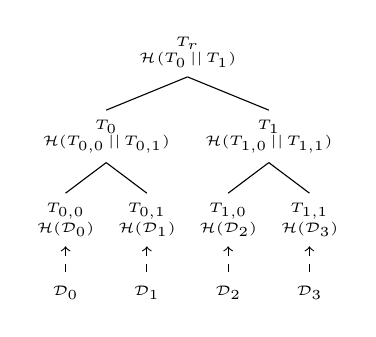
\begin{tikzpicture}
          \tikzset{every tree node/.style={align=center,anchor=north,font=\tiny}}
          \Tree
            [.\node{$T_{r}$ \\ $\hash{T_{0} \concat T_{1}}$};
              [.\node{$T_{0}$ \\ $\mathcal{H}(T_{0, 0} \concat T_{0, 1})$};
                [.{$T_{0, 0}$ \\ $\mathcal{H}(\mathcal{D}_{0})$}
                  \edge[dashed, style={<-}] node {}; $\mathcal{D}_{0}$
                ]
                [.{$T_{0, 1}$ \\ $\mathcal{H}(\mathcal{D}_{1})$}
                  \edge[dashed, style={<-}] node {}; $\mathcal{D}_{1}$
                ]
              ]
              [.\node{$T_{1}$ \\ $\mathcal{H}(T_{1, 0} \concat T_{1, 1})$};
                [.{$T_{1, 0}$ \\ $\mathcal{H}(\mathcal{D}_{2})$}
                  \edge[dashed, style={<-}] node {}; $\mathcal{D}_{2}$
                ]
                [.{$T_{1, 1}$ \\ $\mathcal{H}(\mathcal{D}_{3})$}
                  \edge[dashed, style={<-}] node {}; $\mathcal{D}_{3}$
                ]
              ]
            ]
        \end{tikzpicture}
        \captionsetup{font=scriptsize}
        \caption*{Take $\mathcal{D}_n$ as any data block. A Merkle tree
          can be constructed recursively through the concatenation
          of hashes of a node's children.}
      \end{figure}
    \end{column}
  \end{columns}
\end{frame}

\begin{frame}[plain,noframenumbering]
  \frametitle{Bibliography}
  \bibliographystyle{alpha}
  \bibliography{overview}
\end{frame}

\end{document}
